\documentclass[handout]{beamer}
% \documentclass[mathserif,color=option]{beamer}
% \usepackage{lucida} % Lucida Bright (SO Version)
\usepackage[small]{eulervm} % Euler VM

% This file is a solution template for:

% - Giving a talk on some subject.
% - The talk is between 15min and 45min long.
% - Style is ornate.



% Copyright 2004 by Till Tantau <tantau@users.sourceforge.net>.
%
% In principle, this file can be redistributed and/or modified under
% the terms of the GNU Public License, version 2.
%
% However, this file is supposed to be a template to be modified
% for your own needs. For this reason, if you use this file as a
% template and not specifically distribute it as part of a another
% package/program, I grant the extra permission to freely copy and
% modify this file as you see fit and even to delete this copyright
% notice. 


\mode<presentation>
{
  \usetheme{Antibes}
  % or ... 

  \setbeamercovered{transparent}
  % or whatever (possibly just delete it)
}

\usefonttheme[onlylarge]{structurebold}
\setbeamerfont*{frametitle}{size=\normalsize,series=\bfseries}
\setbeamertemplate{navigation symbols}{}

\usepackage[english]{babel}
% or whatever

\usepackage[latin1]{inputenc}
% or whatever

\usepackage{times}
% \usepackage[T1]{fontenc}
% Or whatever. Note that the encoding and the font should match. If T1
% does not look nice, try deleting the line with the fontenc.

% Change the footnote style
\renewcommand{\thefootnote}{\arabic{footnote}}
\renewcommand{\footnotesize}{\tiny}
\setlength{\skip\footins}{.5cm}

% Use subfigure package
\usepackage{subfigure}

% To display columns dynamically
\usepackage{colortbl}

% drawing trees
% \usepackage{pstricks, pst-node, pst-tree} 

% Put several slides on a single page
% \usepackage{pgfpages}
% \pgfpagesuselayout{2 on 1}[a4paper,border shrink=5mm]

\usepackage{tikz}
\usepackage{amsmath}
\usepackage{amsfonts}
\usepackage{amssymb}
\usepackage{verbatim}
\usetikzlibrary{arrows,shapes}
\usepackage{slashbox, multirow}
\usepackage{array}
\usepackage{url}

% The DeclareGraphicsRule statement causes all file extensions that are not 
% associated with a well-known graphic format to be treated as Encapsulated 
% PostScript files. 
% \usepackage{graphicx}
% \DeclareGraphicsRule{*}{mps}{*}{}

% set caption font style
\usepackage{caption}
\renewcommand{\captionfont}{\scriptsize}
\renewcommand{\captionlabelfont}{\scriptsize}
\setlength{\abovecaptionskip}{3pt}

% For every picture that defines or uses external nodes, you'll have to
% apply the 'remember picture' style. To avoid some typing, we'll apply
% the style to all pictures.
\tikzstyle{every picture}+=[remember picture]

% By default all math in TikZ nodes are set in inline mode. Change this to
% displaystyle so that we don't get small fractions.
\everymath{\displaystyle}

\title[Which Route to Follow?] % (optional, use only with long paper titles)
{Which Route to Follow in Urban Transportation Network?}

\subtitle
{An Introduction to Traveler's Route Choice Behavior} % (optional)

\author[Xiong Y.L.] % (optional, use only with lots of authors)
{Xiong Yiliang}
% - Use the \inst{?} command only if the authors have different
%   affiliation.

\institute[HKPolyU] % (optional, but mostly needed)
{
  Department of Civil and Structural Engineering\\
  Hong Kong Polytechnic University
% - Use the \inst command only if there are several affiliations.
% - Keep it simple, no one is interested in your street address.
}

\date[Mar 1, 2012]
{March 1, 2012}

\subject{Wardrop Equilibrium, Network Design}
% This is only inserted into the PDF information catalog. Can be left
% out. 



% If you have a file called "university-logo-filename.xxx", where xxx
% is a graphic format that can be processed by latex or pdflatex,
% resp., then you can add a logo as follows:

% \pgfdeclareimage[height=0.5cm]{university-logo}{university-logo-filename}
% \logo{\pgfuseimage{university-logo}}



% Delete this, if you do not want the table of contents to pop up at
% the beginning of each subsection:
 \AtBeginSection[]
 {
	\begin{frame}<beamer>{Outline}
	\tableofcontents[currentsection,currentsubsection]
	\end{frame}
 }

%\AtBeginSubsection[]
%{
%  \begin{frame}<beamer>{Outline}
%    \tableofcontents[currentsection,currentsubsection]
%  \end{frame}
%}


% If you wish to uncover everything in a step-wise fashion, uncomment
% the following command: 

%\beamerdefaultoverlayspecification{<+->}

\begin{document}

\begin{frame}
\titlepage

\note{

	Thank all of you for coming to this seminar. I really appreciate this opportunity
	to talk a little about traveler's route choice problem. 
	
	As not everyone in this room work in the field of transportation planning or 
	travel demand modeling, so I try to make this talk as simple as possible. 

}
\end{frame}

\begin{frame}{Outline}
\tableofcontents
  % You might wish to add the option [pausesections]
  
\end{frame}


% Since this a solution template for a generic talk, very little can
% be said about how it should be structured. However, the talk length
% of between 15min and 45min and the theme suggest that you stick to
% the following rules:  

% - Exactly two or three sections (other than the summary).
% - At *most* three subsections per section.
% - Talk about 30s to 2min per frame. So there should be between about
%   15 and 30 frames, all told.

\section{Introduction}

  % - A title should summarize the slide in an understandable fashion
  %   for anyone how does not follow everything on the slide itself.

\subsection{Traffic Congestion}

\begin{frame}{Traffic congestion}

\begin{figure}
\centering
\subfigure[Cross-Harbor Tunnel in Hong Kong]{ 
	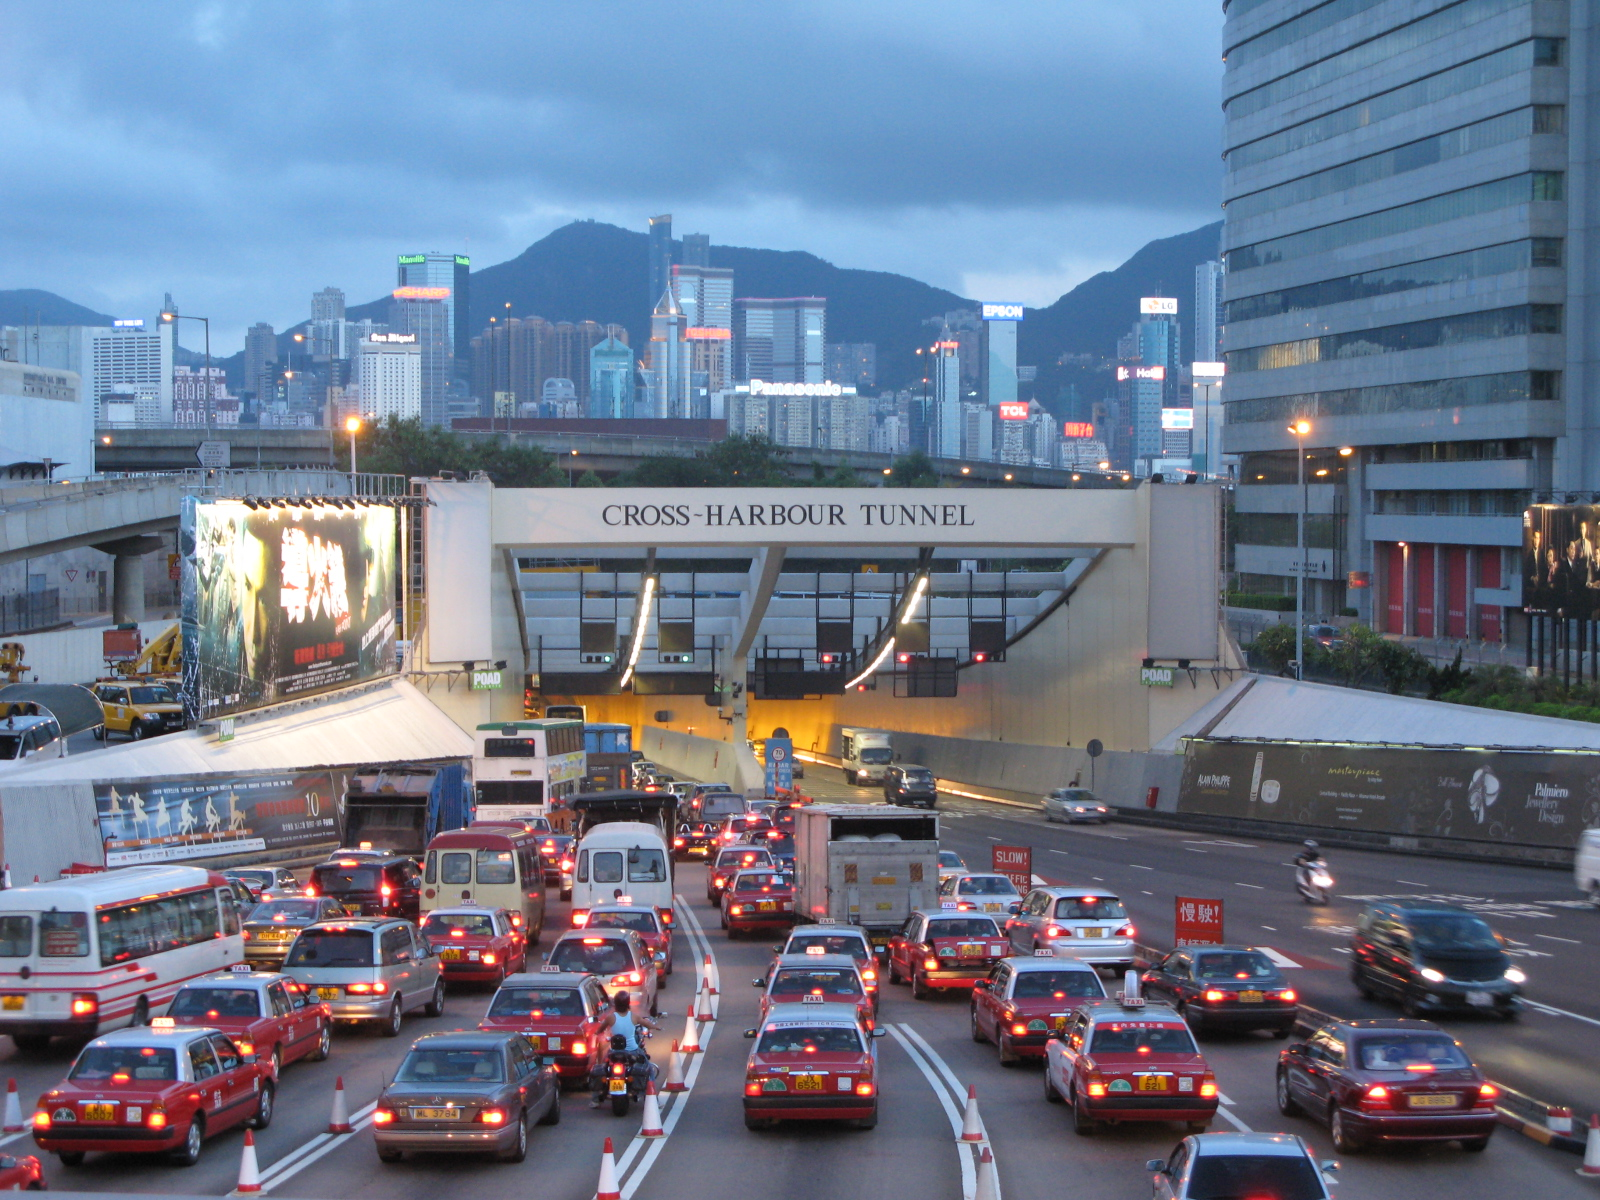
\includegraphics[height=.45\textheight]{fig/HK_Cross_Harbour_Tunnel.jpg}
}%
\subfigure[Heavy traffic in Beijing]{
	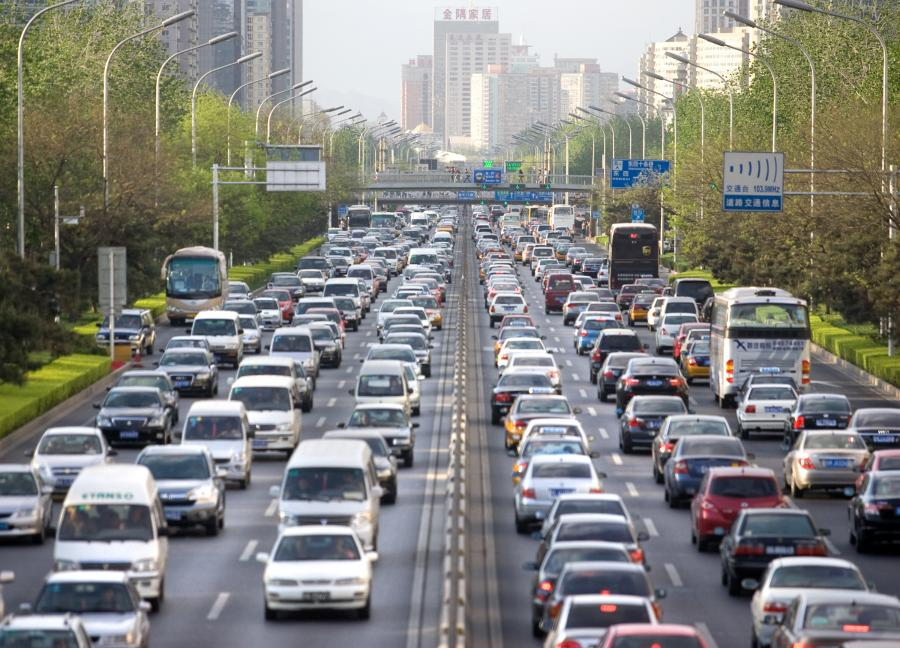
\includegraphics[height=.45\textheight]{fig/Daily-Life-in-Beijing_10.jpg} 
}
\caption{
	Traffic congestion in modern cities
	\footnote{
		The images were downloaded respectively from the Wikipedia 
		(\url{http://en.wikipedia.org/wiki/File:HK_Cross_Harbour_Tunnel.jpg}, 
		visited on July 9, 2010)
		and the United Press International 
		(\url{http://www.upi.com/News_Photos/gallery/Daily-Life-in-Beijing/2012/2}, 
		visited on July 9, 2010). 
	}
}
\end{figure}

\note{

We are all familiar with congested roads, and perhaps also with congestion in 
other networks such as the Internet, so it is obviously important to have a general 
understanding of how and why congestion occurs in networks. The Cross-Harbor 
Tunnel is seriously congested, and the situation is even worse in mainland China. 

}

\end{frame}


\begin{frame}{Non-decreasing travel time}
\uncover<1->{
The travel time of a road depends on the traffic flows on this road: 
\begin{quote}
	The \alert{more vehicles} on a road, the \alert{more time} needed to 
	pass through it. 
\end{quote}
}
\begin{columns}
\column{0.6\linewidth}
\uncover<2->{
Road travel time, $t(x)$, is defined as a \alert{non-decreasing} function of flows $x$. 
\begin{block}{What does \emph{non-decreasing} mean here? }
Mathematically, for any $x_1 > x_2$, we have 
$$t(x_1) \geq t(x_2)$$
\end{block}
}
\column{0.4\linewidth}
% \invisible<1>{
\begin{figure}
\centering
\includegraphics[width=\linewidth]{fig/latency-000}
\caption{Link travel time}
\end{figure}
% }
\end{columns}

\note{

The more vehicles on a link, the more time needed to pass through it. 
Put it mathematically, we get this definition. 

}

\end{frame}

\subsection{A Simple Example}

\begin{frame}{Which route to follow?}
\begin{example}
\begin{figure}
\centering
\includegraphics[width=.45\linewidth]{fig/2-node-000}
\caption{Two roads between $rs$}
\end{figure}
\end{example}
\pause
\begin{block}{Travel Time}
\begin{itemize}
	\item Free travel time on minor road is 20 minutes. 
	\begin{itemize}
		\item The travel time \alert{increases} 5 minutes for each additional vehicle. 
	\end{itemize}
	\item Travel time on highway is \alert{always} 50 minutes. 
\end{itemize}
\end{block}
\end{frame}

\begin{frame}{Flows on a 2-node network}
\begin{columns}
\column{.6\linewidth}
\begin{itemize}
\item The travel time functions: 
\begin{itemize}
	\item Minor road: $ c_{min}(x) = 20 + 5 \cdot x$
	\item Highway: $c_{high}(x) = 50 $
\end{itemize}
\item There are 10 persons traveling between $rs$. 
\uncover<2->{
\item The total travel time for Pattern 1 is
$(3 \times 35 + 7 \times 50) \div 10 = 45.5$
}
\uncover<3->{
\item The total travel time for Pattern 2 is
$(5 \times 50 + 4 \times 50) \div 10 = 50$
}
\end{itemize}
\column{.4\linewidth}
\begin{example}
\begin{figure}
\centering
\includegraphics[width=\linewidth]{fig/2-node-001}
\caption{Traffic Flow Pattern 1}
\end{figure}%
\begin{figure}
\centering
\includegraphics[width=\linewidth]{fig/2-node-002}
\caption{Traffic Flow Pattern 2}
\end{figure}
\end{example}
\end{columns}

\end{frame}

\begin{frame}{All possible traffic flow patterns}

\begin{table}
\small
\centering
\caption{All possible traffic flow patterns}
% \rowcolors[]{1}{blue!20}{blue!10}
\begin{tabular}{%
	r%
	c<{\onslide<1->}!{\vrule}%
	c<{\onslide<1->}%
	c<{\onslide<1->}!{\vrule}%
	l<{\onslide<2->}c%
}
\hline
$x_{min}$ & $x_{high}$ & $t_{min}$ & $t_{high}$ & $\bar{t}$\\
\hline
0 & 10 & 20 & 50 & 50.0 \\
1 & 9 & 25 & 50 & 47.5 \\
2 & 8 & 30 & 50 & 46.0 \\
3 & 7 & 35 & 50 & \textbf{45.5}$^*$ \\
4 & 6 & 40 & 50 & 46.0 \\
5 & 5 & 45 & 50 & 47.5 \\
6 & 4 & 50 & 50 & \textbf{50.0} \\
7 & 3 & 55 & 50 & 53.5 \\
8 & 2 & 60 & 50 & 58.0 \\
9 & 1 & 65 & 50 & 63.5 \\
10 & 0 & 70 & 50 & 70.0 \\
\hline
\end{tabular}\\
\vspace{3pt}
{\scriptsize
	Note: Average travel time $\bar{t} = (x_{min} \cdot t_{min} + x_{high} \cdot t_{high})
	\div (x_{min} + x_{high})$
}
\end{table}

\end{frame}

\begin{frame}{Some insights}
In larger networks, the number of possible traffic flow patterns can be 
\alert{astronomical}. And different patterns result in different network 
performances. 
\pause
\begin{block}{Two questions}
\begin{enumerate}
	\item Which traffic flow pattern is \alert{most likely} to occur in the real world?
	\item What is the \alert{source} of traffic congestion?
\end{enumerate}
\end{block}

\end{frame}

\section{Traffic Equilibrium}

\subsection{Individual's Route Choice Behavior}

\begin{frame}{The shortest path problem}
Every traveler tries to find the \alert{quickest route} between $r$ and $s$.\\
\pause
\begin{minipage}{.4\linewidth}
\begin{block}{Day 1}
\begin{figure}
\centering
% \invisible<1>{ \includegraphics[width=\linewidth]{fig/2-node-003} }
\includegraphics[width=\linewidth]{fig/2-node-003}
\end{figure}
\begin{itemize}
	\item Initially, there is no traveler on the network. 
	\item The \alert{minor road} is the quickest route between $r$ and $s$. 
\end{itemize}
\end{block}
\end{minipage}%
\pause
~$\Rightarrow$~%
\begin{minipage}{.4\linewidth}
\begin{block}{Day 2}
\begin{figure}
\centering
% \invisible<1-2>{ \includegraphics[width=\linewidth]{fig/2-node-004} }
\includegraphics[width=\linewidth]{fig/2-node-004}
\end{figure}
\begin{itemize}
	\item All the travelers crowd into the minor road. 
	\item The \alert{highway} is the quickest route between $r$ and $s$.
\end{itemize}
\end{block}
\end{minipage}%
\pause
~$\Rightarrow$~%
\begin{minipage}{.1\linewidth}
\begin{block}{Day n}
\begin{center}
$\cdots$
\end{center}
\end{block}
\end{minipage}
\end{frame}

\begin{frame}{Complex interaction}

Route Choices \& Route Travel Time:
\begin{itemize}
	\item The travelers attempt to \alert{choose} the quickest route, and this choice
		depends on the \alert{travel time of each route}. 
	\item However, the \alert{route travel time} in turn depends on the 
		\alert{route choices} made by all the travelers in this network. 
\end{itemize}
\pause
\begin{block}{Question}
If this process goes to infinity, is there a \alert{stationary} state or an equilibrium?
\end{block}

\note{

However, the pattern of the flow of traffic through a network is the consequence of 
a subtle and complex interaction between different users. For example, in a road 
network we would normally expect each driver to attempt to choose the most 
convenient route, and this choice will depend upon the delays the driver expects to 
encounter on different roads; but these delays will in turn depend upon the choices of
routes made by others. This mutual interdependence makes it difficult to predict 
the effects of changes to the system, such as the construction of a new road or 
the introduction of tolls in certain places.

If this process goes to infinity, is there a stationary state?
Maybe, this process can reach a state that no one wants to change his route choice
any more.

}

\end{frame}

\subsection{Equilibrium Traffic Flows}

\begin{frame}{Wardrop's Principle}
Each traveler \alert{non-cooperatively} seeks to \alert{minimize} his travel time. 
An equilibrium is reached when no traveler may lower his travel time through 
\alert{unilateral action}. \\
\pause
\begin{block}{Wardrop's Principle}
\begin{quote}
"The journey times on all the routes actually used are \alert{equal}, and \alert{less than}
those which would be experienced by a single vehicle on \alert{any unused route}."~
\footnote{
	Wardrop, J. G., 1952. Some theoretical aspects of road traffic research, 
	Proceedings, Institute of Civil Engineers, Part II, Vol.1, pp. 325-378.
}
\end{quote}
\end{block}
\note{
	An equilibrium is reached when no traveler may lower his travel time by his
	own effect. If he cooperate with others, he may further lower his travel time, 
	but he does not or cannot cooperate with others, the equilibrium is reached. 
}
\end{frame}

\begin{frame}{Find the equilibrium traffic flows}
Wardrop's Principle has two-fold meaning. 
\begin{columns}
\pause
\column{.45\linewidth}
\begin{block}{"The journey times on all the routes actually used are equal."}
At equilibrium, the travel time on minor road is equal to that of highway, 
\begin{align*}
 t_{min} &= t_{high}\\
20 + 5 \cdot x_{min} &= 50 \\
\therefore x_{min} = 6 &\text{ and } x_{high} = 4
\end{align*}
\end{block}
\pause
\column{.45\linewidth}
\begin{block}{"\dots and less than those on any unused route."}
If the number of trips between $r$ and $s$ is 5, all the travelers will choose 
the minor road, because of
\begin{align*}
t_{min}(5) &= 45\\
t_{high}(0) &= 50\\
\therefore t_{min}(5) &< t_{high}(0)
\end{align*}
\end{block}
\end{columns}

\end{frame}

\begin{frame}{Implication of the equilibrium}
\begin{minipage}{.4\linewidth}
\begin{block}{Day 1}
\begin{figure}
\centering
\includegraphics[width=\linewidth]{fig/2-node-003}
\caption{Initial traffic flows. }
\end{figure}
\end{block}
\end{minipage}%
~$\Rightarrow$~%
$\cdots$%
~$\Rightarrow$~%
\begin{minipage}{.4\linewidth}
\begin{block}{Day n}
\begin{figure}
\centering
\includegraphics[width=\linewidth]{fig/2-node-002}
\caption{Equilibrium traffic flows.}
\end{figure}
\end{block}
\end{minipage}
\pause
\begin{block}{Implication of the equilibrium}
If we assume that every traveler chooses the \alert{quickest route}, the traffic flows
that \alert{satisfy Wardrop's Principle} is most likely to occur in real world. 
\end{block}

\note{

This principle helps us understand the underlying travel behavior in urban 
transportation network. And it also provides a method to predict the traffic
flows in the network.

}
\end{frame}

\subsection{Source of Traffic Congestion}

\begin{frame}{Equilibrium flows vs. Optimal flows}
\begin{table}
\centering
\caption{Equilibrium traffic flows are different form optimal flows. }
\small
\begin{tabular}{
	l|p{.1\linewidth}|p{.1\linewidth}|p{.1\linewidth}|p{.1\linewidth}|p{.1\linewidth}
}
\hline
Flows patterns & $x_{min}$ & $x_{high}$ & $t_{min}$ & $t_{high}$ & $\bar{t}$\\
\hline
Optimal flows & 3 & 7 & 35 & 50 & 45.5$^*$ \\
Equilibrium flows & 6 & 4 & 50 & 50 & 50.0 \\
\hline
\end{tabular}\\
\vspace{3pt}
{\scriptsize
	Note: $\bar{t} = (x_{min} \cdot t_{min} + x_{high} \cdot t_{high})
	\div (x_{min} + x_{high})$
}
\begin{itemize}
	\item Compared to optimal flows, \alert{too many} travelers crowd into 
		the minor road in equilibrium flows. 
	\item The average travel time of equilibrium flows is 4.5 minutes 
		\alert{larger than} that of optimal equilibrium. 
\end{itemize}
\pause
\begin{block}{Source of traffic congestion}
\begin{center}
Choosing quickest route $\Rightarrow$%
Crowding effects $\Rightarrow$%
Traffic congestion
\end{center}
\end{block}
\end{table}

\end{frame}

\section{Summary}

\begin{frame}{Summary}
  % Keep the summary *very short*.
Investigate the traffic congestion in light of travelers' route choice behaviors: 
\begin{description}
	\item[Individual's behavior] The quickest path problem.
	\item[Aggregate quantity] Equilibrium traffic flow. 
	\item[Macroscopic phenomenon] Traffic congestion. 
\end{description}

  \note{ 
  The main contributions of this research are that in addition to accounting for traveler's 
  heterogeneity in preference and perceptions, it also
  investigates probabilistic activity/travel behaviors in uncertain environment. This can help us
  to understand the source of uncertainty in the demand side of urban transportation system. 
  }
  
\end{frame}

\begin{frame}{State-of-the-Art Research}
Considerable number of studies have emerged in recent years: 
\begin{itemize}
	\item Road congestion pricing
	\item Random errors in travelers' choices
	\item Uncertainties in travel time
	\item $\dots$
\end{itemize}
\end{frame}

\appendix
%
%\section{Transportation Network Design}
%
%\begin{frame}{Transportation Network Design}
%$\dots$
%\end{frame}

\section*{Appendix}

\begin{frame}{Network Structure}

\begin{columns}
\column{.6\linewidth}
An abstract model for urban transportation network:
\begin{itemize}
	\item A set of nodes $N$, and a set of links $A$. 
	\item Origin-destination (O-D) pair $rs$, where $r,s \in N$. 
	\item Number of trips made between each O-D pair $f^{rs}$. 
	\item For each link $a \in A$, a travel time function $t_a(x_a)$ is given.
\end{itemize}
\column{.4\linewidth}
\begin{example}
\begin{figure}
\centering
\includegraphics[width=\linewidth]{fig/braess-000}
\caption{Braess's network}
\end{figure}
\end{example}
\end{columns}

\end{frame}

\end{document}
